\documentclass[10pt]{article}

\def\Type{LessonCaelan}
\def\TypeNum{Lesson 14}
\def\TypeTitle{Applied Optimization\\Extra Practice KEY }
\def\Semester{Fall 2021} %Not Used 
\def\Course{MATH 1190 \& 1210}
\def\Targets{  {\bf\color{RedOrange}A3} }

\usepackage{preambleDJ}

%\usepackage{ragged2e}


%%%%%%%%%%%% BEGIN DOCUMENT %%%%%%%%%%%%%%%
%%%%%%%%%%%% BEGIN DOCUMENT %%%%%%%%%%%%%%%
%%%%%%%%%%%% BEGIN DOCUMENT %%%%%%%%%%%%%%%
%%%%%%%%%%%% BEGIN DOCUMENT %%%%%%%%%%%%%%%
%%%%%%%%%%%% BEGIN DOCUMENT %%%%%%%%%%%%%%%

\begin{document}

\pagestyle{otherpages}
\thispagestyle{firstpage}
\vs{.5}


\exercise{\target{A3}} An architect is designing a large window for renovations in Clemons library.  The window is composed of a rectangle and a half of a circular disc.  To keep costs down, the perimeter of the window must be exactly $30$ feet.  What dimensions will allow the greatest amount of light into the building?\\


\mpageT{.2}{.9}{
\textbf{Modeling Phase:}\\
\vs{-.35}\graphicsL{windowKey}{1.5}{\hs{.3}Figure 1}
}{
\tasksA{2}{
\task Setup a function that describes the amount of light entering the window using the variables shown  in Figure 1.  {\em Hint}: How is the``amount of light" related to the shape of the window?
\sol{
The area of the window will determine how much light will enter the building.
\al{
A&=A_{rectangle}+A_{halfCircle}
\intertext{Since the radius of the circle is half the width of the rectangle, thus $width=2r$}
A_{rectangle}&=height\times width=h\cdot 2r\\
A_{halfCircle}&=\frac{1}{2}\pi r^2
\intertext{Thus,}
A&=2rh+\frac{\pi r^2}{2}
}
}
\task  Setup an expression that translates `` the perimeter of the window must be exactly $30$ feet" into  a math equation using the variables shown  in Figure 1. 
\sol{
The perimeter consists of $3$ sides of the rectangle and the length of the boundary of the half circle. 
\al{
P&=h+2r+h+\pi r\\
P&=2h+2r+\pi r
\intertext{We're told that the perimeter must be $30$ feet, so}
30&=2h+2r+\pi r
}
}
}
}
 \tasksAS{2}{3}{
\task* Identify which quantity from $(a)$ and $(b)$ we are trying to minimize or maximize. It will contain variables $r$ and $h$. Use the remaining quantity and solve for one of those variables and then substitute into the first equation. This will reduce it to a function of only one variable.
\sol{
We want to maximize the amount of light, so we're going to maximize area. But since $A$ is a function of both $r$ and $h$, we need to reduce this to a function of only one variable.  We can use the perimeter to solve for either variable.  It's easier to solve for $h$.  
\al{
2h+2r+\pi r&=30\\
2h &=30-2r-\pi r\\
h&=\frac{30-2r-\pi r}{2}\\
h&=\frac{30}{2}-\frac{2r}{2}-\frac{\pi r}{2}\\
h&=15-r-\frac{\pi r}{2}
}
Thus 
\al{
A&=2rh+\frac{\pi r^2}{2}\\
&=2r (15-r-\frac{\pi r}{2})+\frac{\pi r^2}{2}\\
&=30r-2r^2-\pi r^2+\frac{\pi r^2}{2}\\
A&=30r-2r^2-\frac{\pi r^2}{2}
}
}
}



\textbf{Calculus Phase:}
%\tasksAS{2}{4}{
\enumA{\setItemnumber{4}
\item Find critical number(s) of your new function of one variable. Your answer will involve the number $\pi$.
\sol{
\al{
A^{\prime}(r)&=30-4r-\pi r\\
A^{\prime}(r)&=30-r(4+\pi)
}
There are two situations that generate critical numbers 
\itemI{
\item $A^{\prime}(r)=DNE$. This occurs when we have a division by $0$, $\sqrt{(-)}$, $\ln(0)$ or $\ln(-)$.  There is no value of $r$ that will create any of these.   
\item $A^{\prime}(r)=0$.
\al{
 A^{\prime}(r)&=0\\
 30-r(4+\pi)&=0\\
- r(4+\pi)&=-30\\
r&=\frac{-30}{-(4+\pi)}\\
r&=\frac{30}{4+\pi} \approx 4.2 \text{ feet}
}
}\vs{-.2}
%Thus we have one critical number, $\ds r=\frac{30}{4+\pi} \approx 4.2$ feet
}
\item  Determine if your critical number(s) are an absolute maximum/minimum(s).
\sol{
To determine absolute max/min, we need a domain. $r$ must be positive since it doesn't make sense to have a negative radius nor a radius of $0$.  Thus the domain is $0<r<\infty$. We only have one critical number on this domain, $\ds r=\frac{30}{4+\pi} \approx 4.2$ feet.  \\
\\
In order to determine if our critical point is a local min, max or neither, we find the sign of the derivative before and after our critical number.  
\itemI{
\item Let's choose a number less than $\ds \frac{30}{4+\pi} \approx 4.2$, say $r=3$.
\al{
A^{\prime}(3)=30-3(4+\pi) \approx +8.58
}\vs{-.3}
\item Let's choose a number greater than $\ds \frac{30}{4+\pi} \approx 4.2$, say $r=5$.
\al{
A^{\prime}(5)=30-5(4+\pi) \approx -5.71
}
}
A sign chart collects all of this information.
\begin{center}
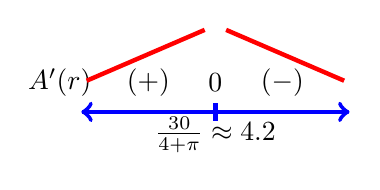
\begin{tikzpicture}
    \begin{axis}[
    	axis x line=none,
	            axis y line=none,
		x label style={anchor=west},
            xlabel={},
            xtick       = {0},
            xticklabels = {$c$},
            y label style={anchor=south},
            ylabel={},
            ytick       = {-6,-4,-2,2,4,6},
            yticklabels = {$-6$,$-4$,$-2$,$2$,$4$,$6$},
            samples     = 320,
            domain      = -2.5:2.5,
            restrict y to domain=-6.5:6.5,
            xmin = -3.5, xmax = 3.5,
            ymin = -6.5, ymax = 6.5,
            width=2.5in, height=2.5in,
            grid=none, grid style=solid
          ]
    \addplot[domain=-2.5:2.5, blue, ultra thick, mark=none, <->]{0)};
   \draw (-2.9,1) node{$\Large A^{\prime}(r)$};
   \draw[ultra thick, blue] (0,.3)--(0,-.3);
      \draw (0,-.8) node{$\frac{30}{4+\pi}\approx 4.2$};
            \draw (0,1) node{$0$};
            \addplot[domain=-2.4:-.2, red, ultra thick, mark=none, -]{2*x/2.5+3)};
                        \addplot[domain=0.2:2.4, red, ultra thick, mark=none, -]{-2*x/2.5+3)};
                             \draw (-1.25,1) node{\blue{$(+)$}};
                              \draw (1.25,1) node{\blue{$(-)$}};
    \end{axis}
\end{tikzpicture}  
\end{center}
We see that we have a {\em local maximum} by the First Derivative Test. \\

However since we have only one critical number on the domain and it's a local maximum, the First Derivative Test for Absolute Extrema sez that this is also the {\em absolute maximum}.\\

Thus the radius of the half-circle that lets in the maximum amount of light is $\ds r=\frac{30}{4+\pi} \approx 4.2 \text{ feet}$ and the height of the rectangular portion of the window is 
\al{
h&=15-r-\frac{\pi r}{2}\\
h&=15-\frac{30}{4+\pi}-\frac{\pi (\frac{30}{4+\pi})}{2}\approx 17.40\text{ feet}
}
}
}

\newpage 

\exercise{\target{A3}} An architect is designing a large window for renovations in Clemons library.  The window is composed of a rectangle and a half of a circular disc.  To allow enough light into the library the window must have a total area of exactly $100$ feet$^2$. The cost of materials varies
\itemI{
\item The frame for the half-disc costs $\$20$ per foot.
\item The frame for the  sides of the rectangle cost $\$10$ per foot
}
Find the dimensions that minimize the cost.

\mpageT{.2}{.9}{
\textbf{Modeling Phase:}\\
\vs{-.35}\graphicsL{windowKey}{1.5}{\hs{.3}Figure 2}
}{
\tasksA{2}{
\task Setup a function that describes the cost of the window frame using the variables shown  in Figure 2.  
\sol{
The cost of the frame for the rectangular part of the window is 
\al{
C_{rectangle}&=\text{ cost per foot} \times \#\text{ feet}\\
&=\$10 (h+2r+h)\\
&=\$10(2h+2r)\\
&=20h+20r
}
The cost of the frame for the half-circle is 
\al{
C_{halfCircle}&=\text{ cost per foot} \times \#\text{ feet}\\
&=\$20 \cdot \pi r
}
\al{
C&=C_{rectangle}+C_{halfCircle}\\
C&=20h+20r+20\pi r
}
}
\task  Setup an expression that translates ``the window must have a total area of exactly $100$ feet$^2$." into  a math equation using the variables shown  in Figure 2. 
\sol{ The width of the rectangle is twice the radius, $width=2r$.
\al{
A&=A_{rectangle}+A_{halfCircle}\\
&=h(2r)+\frac{\pi r^2}{2}
\intertext{We are told that the area must be exactly $100ft^2$, so }
100&=2hr+\frac{\pi r^2}{2}
}
}
}
}
\tasksAS{2}{3}{
\task* Identify which quantity from $(a)$ and $(b)$ we are trying to minimize or maximize. It will contain variables $r$ and $h$. Use the remaining quantity and solve for one of those variables and then substitute into the first equation. This will reduce it to a function of only one variable.
\sol{
We would like to minimize the cost. However the cost function involves both of the variables $r$ and $h$. In order to find a derivative, we need to reduce this to a function of only one variable. To do this, we utilize our Area equation to solve for either $r$ or $h$. It is easier to solve for $h$.
\al{
2hr+\frac{\pi r^2}{2}&=100\\
2hr&=100-\frac{\pi r^2}{2}\\
h&=\frac{100-\frac{\pi r^2}{2}}{2r}\\
h&=\frac{100}{2r}-\frac{\frac{\pi r^2}{2}}{2 r}\\
h&=\frac{50}{r}-\frac{\pi r}{4}
}
Now substitute this for $h$ in our Cost function
\al{
C&=20h+20r+20\pi r\\
C&=20\left(\frac{50}{r}-\frac{\pi r}{4} \right)+20r+20\pi r\\
C&=\frac{100}{r}-\frac{20 \pi r}{4}+20r +20\pi r\\
C&=\frac{100}{r}-5 \pi r +20r+20\pi r\\
C&=\frac{100}{r} +20r+15\pi r\\
}
}
}
\textbf{Calculus Phase:}
\enumA{\setItemnumber{4}
\item Find critical number(s) of your new function of one variable. Your answer will involve the number $\pi$.
\sol{
We first find the derivative 
\al{
C(r)&=\frac{100}{r} +20r+15\pi r=100 r^{-1}\\
&=100r^{-1} +20r+15\pi r\\
C^{\prime}(r)&=-100r^{-2} +20+15\pi\\
&=-\frac{100}{r^2}+20+15\pi
}
We must check two conditions in order to identify critical numbers.
\itemI{
\item $C^{\prime}(r)=DNE$.  When $r=0$ we have a division by $0$ which means $C^{\prime}(0)$ DNE. Thus $r=0$ could be a critical number. However, $r=0$ is not in the domain of $C(r)$ since $\ds C(0)=\frac{100}{0} +20\cdot 0+15\pi r\cdot 0$ contains a division by $0$. Thus we ignore $r=0$.
\item $C^{\prime}(r)=0$ 
\al{
C^{\prime}(r)&=0\\
-\frac{100}{r^2}+20+15\pi&=0\\
-\frac{100}{r^2}&=-20-15\pi\\
-100&=r^2(-20-15\pi) \text{ (after multiplying both sides by $r^2$)}\\
\frac{-100}{-20-15\pi}&=r^2\\
\frac{-5\cdot 20}{-5\cdot (4+3\pi)} &=r^2\text{ (after factoring $-5$ out of all terms)}\\
\frac{ 20}{4+3\pi}&=r^2 \\
\pm \sqrt{\frac{20}{4+3\pi}} &\approx r
}
}
Our two critical numbers are $\ds r=\pm \sqrt{\frac{20}{4+3\pi}} \approx \pm 1.49 $
}
\item  Determine if your critical number(s) are an absolute maximum/minimum(s).
\sol{
To find absolute max/mins we need a domain. The radius $r$ must be positive since it doesn't make sense to have a negative or $0$ radius. The domain is $0<r<\infty$. \\

We eliminate $\ds r=-\sqrt{\frac{20}{4+3\pi}}$ as a critical number since it's not in the domain. Thus we test $\ds r=\sqrt{\frac{20}{4+3\pi}} \approx 1.49$ to see if it is a local max, min or neither. 
\itemI{
\item We choose a point to the left of $r=1.49$ say $r=1$
\al{
C^{\prime}(1)=-\frac{100}{1^2}+20+15\pi=-80+15\pi\approx-32.88
}
\item We choose a point to the right of $r=1.49$ say $r=2$
\al{
C^{\prime}(2)=-\frac{100}{2^2}+20+15\pi=-25+20+15\pi\approx +42.12
}
}
The sign chart below captures this information and we see that we have a {\em local minimum} by the First Derivative Test.
\begin{center}
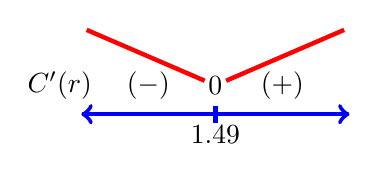
\begin{tikzpicture}
    \begin{axis}[
    	axis x line=none,
	            axis y line=none,
		x label style={anchor=west},
            xlabel={},
            xtick       = {0},
            xticklabels = {$c$},
            y label style={anchor=south},
            ylabel={},
            ytick       = {-6,-4,-2,2,4,6},
            yticklabels = {$-6$,$-4$,$-2$,$2$,$4$,$6$},
            samples     = 320,
            domain      = -2.5:2.5,
            restrict y to domain=-6.5:6.5,
            xmin = -3.5, xmax = 3.5,
            ymin = -6.5, ymax = 6.5,
            width=2.5in, height=2.5in,
            grid=none, grid style=solid
          ]
    \addplot[domain=-2.5:2.5, blue, ultra thick, mark=none, <->]{0)};
   \draw (-2.9,1) node{$\Large C^{\prime}(r)$};
   \draw[ultra thick, blue] (0,.3)--(0,-.3);
      \draw (0,-.7) node{$1.49$};
        \draw (0,1) node{$0$};
            \addplot[domain=-2.4:-.2, red, ultra thick, mark=none, -]{-2*x/2.5+1)};
                        \addplot[domain=0.2:2.4, red, ultra thick, mark=none, -]{2*x/2.5+1)};
                             \draw (-1.25,1) node{\blue{$(-)$}};
                              \draw (1.25,1) node{\blue{$(+)$}};
    \end{axis}
\end{tikzpicture}
\end{center}

We still need to determine if our local minimum is also an absolute minimum.  Since we only have one critical number on the domain $0<r<\infty$ and we just found that it's a local minimum, the First Derivative Test for Absolute Extrema says that it's also the absolute minimum.\\
\\
We thus minimize cost when the radius is $$r=\pm \sqrt{\frac{20}{4+3\pi}} \approx \pm 1.49 \text{ feet}$$
The height of the rectangular portion is 
\al{
h&=\frac{50}{r}-\frac{\pi r}{4}\\
h&=\frac{50}{\sqrt{\frac{20}{4+3\pi}} } -\frac{\pi \sqrt{\frac{20}{4+3\pi}} }{4}\\
h&\approx 40.01 \text{ feet}
}
}
}



\end{document}
